\chapter{Progettazione della soluzione}\label{chap:Progettazione della soluzione}

La soluzione proposta è stata progettata con l'obiettivo di renderla indipendente sia dal tipo di deployment presentato ad essa, sia dal tipo di architettura Kubernetes. Uno degli obiettivi preposti sin dall'inizio dello sviluppo è stato infatti quello di consentirne l'utilizzo indipendentemente dal tipo di architettura Kubernetes in esecuzione sul cluster (per esempio Minikube\footnote{https://minikube.sigs.k8s.io/docs/}, kind\footnote{https://kind.sigs.k8s.io} o servizi cloud). Inoltre, l'approccio proposto è di tipo \myenquote{black-box}, quindi è progettato specificatamente per non accedere/modificare il codice dei microservizi che formano un'applicazione. Quanto presentato qui di seguito è stato quindi essenziale per raggiungere gli obiettivi descritti sopra.

\section{Separazione delle risorse in namespace dedicati}\label{sect:Spostamento delle risorse in namespace dedicati}
L'orchestrazione di applicazioni basate su microservizi con Kubernetes, richiede una gestione efficace delle risorse e una segmentazione chiara delle funzionalità. Per questo motivo, sono stati definiti tre nuovi namespace:
\begin{itemize}
\item \texttt{log-enabled:} Namespace dedicato alle risorse e ai servizi dell'applicazione di cui si vogliono ottenere, raccogliere e analizzare i log.
\item \texttt{log-istio-system:} Namespace dedicato ai componenti della rete Service Mesh di Istio.
\item \texttt{log-elk:} Namespace dedicato ai componenti dello stack ELK.
\end{itemize}



Questo approccio a namespace separati non solo mira a preservare l'integrità del dispiegamento originale, richiedendo di applicare solo modifiche minimali al file di deployment, ma fornisce uno spazio separato da tutto il resto del cluster, e dedicato unicamente per le operazioni di logging e analisi. Questa scelta si manifesta in diversi vantaggi:
\begin{itemize}
\item \textbf{Completo isolamento:} Come specificato, un namespace fornisce completo isolamento dai servizi che si trovano su altri namespace. Su Kubernetes, infatti, eventuali accessi inter-namespace possono solamente essere gestiti tramite il cosiddetto RBAC (Role-Based Access Control).
\item \textbf{Possibilità di sovrapposizione dei nomi di identificazione:} Servizi con nomi identici possono infatti coesistere sullo stesso cluster, purché essi si trovino su namespace differenti.
\item \textbf{Possibilità di sovrapposizione di numeri di porta:} Due servizi, residenti in namespace differenti, possono usare gli stessi numeri di porta per comunicare con i rispettivi destinatari, evitando quindi conflitti o interferenze.
\item \textbf{Gestione semplificata delle risorse:} Avendo namespace specifici per ogni funzione, è più facile allocare, gestire e limitare le risorse (come CPU, memoria, e storage) per ogni servizio o applicazione.
\item \textbf{Politiche di sicurezza specifiche:} Con la separazione dei namespace, è possibile definire politiche di accesso e sicurezza dedicate per ciascun ambiente.
\item \textbf{Facilità di monitoraggio:} Ogni namespace può avere metriche e dashboard dedicati, permettendo un monitoraggio più granulare e specifico.
\item \textbf{Scalabilità indipendente:} Ogni namespace può essere scalato in base alle proprie esigenze, senza influenzare gli altri namespace.
\end{itemize}

Sia per far fronte alla necessità di poter analizzare interazioni tra applicazioni che sfruttano più namespace contemporaneamente, che anche per analizzare più applicazioni allo stesso tempo, nell'implementazione è stata prevista una funzionalità che permette di specificare un suffisso per il namespace di destinazione, tipicamente riempito con il nome dell'applicazione che si vuole analizzare. Utilizzando questa opzione, il namespace di destinazione sarà del tipo \texttt{log-enabled-suffix}. Trattandosi di un'opzione facoltativa, per brevità nelle sezioni successive sarà trattato unicamente il namespace \texttt{log-enabled}, ma è importante tenere presente che ogni funzionalità che è riferita a tale namespace, è sempre applicabile anche ai namespace del tipo \texttt{log-enabled-suffix}.



\section{Configurazione della rete Istio}

\subsection{Configurazione dell'access logging}
L'interazione tra Istio e Envoy in relazione all'access logging può essere vista come una sinergia tra il controllo di livello superiore fornito da Istio e le capacità operative e dettagliate offerte da Envoy. Istio, attraverso la sua interfaccia di controllo centralizzato, permette una configurazione dell'access logging facile e uniforme per tutti i servizi che compongono la mesh. Tale configurazione viene poi tradotta e applicata in modo efficiente dal proxy Envoy, che si occupa della cattura effettiva dei log e del loro inoltro alle destinazioni designate.

Per la soluzione proposta, il formato di access logging desiderato è mostrato nel Codice \ref{lst:access_log_format}, e tale scelta è motivata dalla necessità di ricavare tutte le informazioni necessarie a yRCA \cite{tesi_spiridioni}.

\begin{lstlisting}[caption={Formato richiesto per l'ottenimento dell'access logging.}, label=lst:access_log_format, keywordstyle=\color{black}, commentstyle=\color{black},stringstyle=\color{black},numberstyle=\color{black}]
{
        "start_time": "%START_TIME%",
        "response_code": "%RESPONSE_CODE%",
        "response_flags": "%RESPONSE_FLAGS%",
        "response_code_details": "%RESPONSE_CODE_DETAILS%",
        "duration": "%DURATION%",
        "request_duration": "%REQUEST_DURATION%",
        "request_tx_duration": "%REQUEST_TX_DURATION%",
        "response_duration": "%RESPONSE_DURATION%",
        "response_tx_duration": "%RESPONSE_TX_DURATION%",
        "authority": "%REQ(:AUTHORITY)%",
        "x-request-id": "%REQ(X-REQUEST-ID)%"
      }
\end{lstlisting}
Ogni campo ha una precisa motivazione e funzionalità:
\begin{itemize}
\item \texttt{"start\_time"}: Questo campo indica l'orario di inizio di una richiesta, in termini di ora, minuto, secondo e millisecondo. Il formato utilizzato è l'ISO 8601.

\item \texttt{"response\_code"}: Rappresenta il codice HTTP inviato in risposta ad una richiesta. Questo campo può anche essere \myenquote{0}: in tal caso, significa che il servizio invocato non ha mai inviato la risposta. Solitamente, questo significa che il client si è disconnesso.

\item \texttt{"response\_flags"}: Questi flag forniscono informazioni aggiuntive sulla risposta, come ad esempio se è stata terminata prematuramente o se ci sono stati problemi nella connessione. Per la rielaborazione dei log nel formato per yRCA, vengono usati questi codici:

\begin{itemize}
\item \texttt{UF:} In aggiunta al codice di risposta 503, indica un fallimento nella connessione da parte del servizio chiamato.
\item \texttt{UC:} In aggiunta al codice di risposta 503, indica la terminazione della connessione da parte del servizio chiamato.
\item \texttt{DC:} In aggiunta al codice di risposta 504, indica la terminazione della connessione da parte del servizio chiamante.
\item \texttt{UT:} In aggiunta al codice di risposta 504, indica un evento di timeout da parte del servizio chiamato.
\end{itemize}

\item \texttt{"response\_code\_details"}: Fornisce dettagli sul codice di risposta, come ad esempio se è stato causato da un filtro specifico.

\item \texttt{"duration"}: Durata totale della richiesta del servizio chiamante, dal momento in cui viene ricevuta fino a quando viene inviata la risposta. Questo campo è espresso in millisecondi.

\item \texttt{"request\_duration"}: Tempo totale dallo \texttt{start\_time} al momento in cui l’ultimo byte viene ricevuto dal client, in millisecondi.

\item \texttt{"request\_tx\_duration"}: Tempo totale dallo \texttt{start\_time} al momento in cui l’ultimo byte viene inviato al servizio chiamato, in millisecondi.

\item \texttt{"response\_duration"}: Tempo totale dallo \texttt{start\_time} al momento in cui il primo byte viene letto dal servizio chiamato, in millisecondi.

\item \texttt{"response\_tx\_duration"}: Tempo totale dal momento in cui il primo byte viene letto dal servizio chiamato al momento in cui l’ultimo byte viene mandato al servizio chiamante.

\item \texttt{"authority"}: L'autorità di richiesta, spesso l'host HTTP. È usata per distinguere una richiesta da una risposta.

\item \texttt{"x-request-id"}: L'UUID univoco assegnato alla richiesta. Si tratta di un campo popolato dai proxy Envoy.

\end{itemize}

In casi più rari, però, ci possono essere problemi che impediscono il corretto funzionamento dell'intero pod, facendo quindi attendere il servizio chiamante un tempo indefinito in attesa di una risposta dal proxy Envoy. È necessario quindi un sistema che rilevi questo comportamento e lo interrompa, generando un messaggio di timeout. Il componente che è trattato nel paragrafo seguente è di cruciale importanza per questo scopo.


\subsection{Rilevamento dei Timeout}\label{subsect:Istio Virtual Service}
La capacità di rilevamento dei timeout è essenziale quando si tratta di analizzare fallimenti in un ambiente a microservizi. I timeout, infatti, rappresentano uno dei meccanismi chiave per identificare problemi come la latenza eccessiva, il sovraccarico di un servizio o semplicemente la mancata risposta da parte di un servizio downstream. In un sistema altamente distribuito come una mesh di servizi, il rilevamento e la gestione tempestiva dei timeout possono prevenire la propagazione di errori, migliorando la resilienza complessiva dell'applicazione.

In questo contesto, si cerca di rilevare un eventuale timeout sfruttando delle funzionalità messa a disposizione dalla rete mesh Istio.
È infatti possibile ottenere tale funzionalità tramite il concetto di \textit{VirtualService}, componente inizialmente progettato per definire e configurare le regole di routing per il traffico, ma che permette inoltre di specificare regole per la personalizzazione del tempo di timeout nelle chiamate tra microservizi differenti.

Si noti che un VirtualService non è una vera e propria entità presente in un cluster Kubernetes. Quest'ultimo è unicamente un concetto astratto che rappresenta una precisa configurazione che Istiod applica ai proxy Envoy (e, se presente nella rete, anche ad altra componentistica come l'\textit{Ingress} o \textit{Egress Gateway}). Una volta applicata la configurazione a Istiod, sarà quest'ultimo a configurare automaticamente il sidecar Envoy per il funzionamento desiderato, e a controllare periodicamente che lo stato del sistema attuale sia allineato con le configurazioni fornite.

Il Codice \ref{lst:istio_virtualservice} mostra come si presenta il file di configurazione per un VirtualService, configurato unicamente per la rilevazione di timeout.

\begin{lstlisting}[caption={Istio VirtualService per la rilevazione di timeout.}, label=lst:istio_virtualservice, keywordstyle=\color{black}, commentstyle=\color{black},stringstyle=\color{black},numberstyle=\color{black}, escapechar=|]
apiVersion: networking.istio.io/v1alpha3
kind: VirtualService
metadata:
  name: <nome del VirtualService>
  namespace: log-enabled
spec:
  hosts:
  - <nome del servizio di origine>
  http:
  - route:
    - destination:
        host: <nome del servizio di destinazione>
    timeout: 15s
\end{lstlisting}

\begin{itemize}
    \item \texttt{apiVersion:} Definisce la versione dell'API di Kubernetes. Da notare che la versione API indica l'utilizzo di una risorsa di Istio, e non nativa Kubernetes.
    \item \texttt{kind:} Specifica il tipo di risorsa, qui \myenquote{VirtualService}.
    \item \texttt{metadata - name:} Il nome del VirtualService. Nel contesto di questo progetto, tutti i VirtualService mantengono lo stesso nome del servizio a cui si riferiscono.
    \item \texttt{metadata - namespace:} Namespace, qui \myenquote{log-enabled}, in quanto si tratta di un componente che andrà dispiegato in quel namespace.
    \item \texttt{spec - hosts:} Elenca i servizi di origine per questo VirtualService. Nel contesto del progetto, ogni VirtualService viene assegnato unicamente ad uno e un solo Service Kubernetes.
    \item \texttt{spec - http - route - destination - host:} Nome del servizio di destinazione. Non essendoci particolari regole di routing, in questa sezione è specificato un solo host di destinazione, ovvero il servizio originale.
    \item \texttt{spec - http - route - timeout:} In questa sezione è configurato il timer con il quale il VirtualService deve emettere un messaggio di timeout. Di default, la soluzione prevede 15 secondi di timeout, ma lascia all'utente la possibilità di configurare questo periodo. Le informazioni sulla configurabilità di questo periodo saranno trattate nel Capitolo \ref{chap:Realizzazione della soluzione}.
\end{itemize}

\section{Configurazione dello stack ELK}

Come illustrato nel Capitolo \ref{chap:Fondamenti Teorici}, lo stack ELK, composto da ElasticSearch, Logstash e Kibana, con l'aggiunta di Filebeat per la collezione dei log, rappresenta una soluzione consolidata per la gestione, l'analisi e la visualizzazione dei log generati dalle applicazioni. Nel contesto di questo progetto, la centralità dello stack ELK non si limita alla raccolta e visualizzazione dei log, ma si estende ad un ruolo strategico nell'identificazione e nell'analisi dei fallimenti.

\subsection{Flusso di raccolta ed elaborazione dei log}
L'intero processo di raccolta, elaborazione, e memorizzazione dei log è basato sull'interazione tra i sistemi dello stack ELK, ed è stato progettato sin dall'inizio con l'idea di essere il più possibile scalabile, per far fronte anche a possibili carichi di lavoro più pesanti del previsto. Il processo avviene come segue:
\begin{enumerate}
\item Filebeat monitora continuamente il path \verb|/var/log/containers|, in tutti i nodi del cluster. Questo è il path standard dove vengono memorizzati i log dei cluster Kubernetes \cite{kubernetes_log_location}.
\item All'aggiunta di una nuova linea di log, Filebeat la raccoglie ed aggiunge ad essa metadati di Kubernetes. Questi metadati includono ad esempio il nome del pod, il nome del container, e il nome del worker node che eseguiva il pod.
\item I log vengono poi inviati all'istanza di Logstash, in esecuzione sullo stesso namespace.
\item Logstash raccoglie i log e, tramite un filtro JSON, riesce a rendere il più conforme possibile log di \verb|istio-proxy|, ed eventualmente anche log di applicazioni che emettono log in formato JSON, al formato ECS (Elastic Common Schema). I dettagli sull'utilizzo e le motivazioni di questo filtro saranno trattati al Capitolo \ref{subsect:Configurazione di Logstash}.
\item I log vengono poi inviati all'istanza di ElasticSearch.
\item ElasticSearch esegue quello che è chiamato \myenquote{\textit{dynamic mapping}}, creando automaticamente una mappa dei campi presenti nel log in base al loro tipo di dato. Questo permette di ottimizzare le query di ricerca e di analisi dati che saranno eseguite sull'istanza in un secondo momento.
\item Una volta archiviati su ElasticSearch, i log sono immediatamente disponibili per le operazioni di ricerca, visualizzazione e analisi. Questo rende particolarmente agevole e veloce l'individuazione di possibili problemi o anomalie all'interno del cluster.
\end{enumerate}
Inoltre, si prevede l'utilizzo di uno script per ottenere un dump dei log memorizzati nell'istanza ElasticSearch. Tale script deve consentire il download dei log, incluso il formato GELF (\textit{Graylog Extended Format}) atteso in input da yRCA.

\subsection{Configurazione di Filebeat}
La scelta di utilizzare Filebeat come collettore di log è motivata dal voler rendere il processo di raccolta dei log meno oneroso in termini di risorse. Infatti, nonostante Logstash possegga al suo interno capacità di collezione di log da file, esso necessita di molte più risorse, se comparato a Filebeat \cite{filebeat_resources}. Ad esempio, su un cluster multi-nodo, l'esecuzione di un'istanza di Logstash su ogni nodo (necessaria per collezionare log da tutti i pod) comporterebbe un overhead maggiore rispetto a Filebeat. Filebeat, invece, è un collettore di metriche progettato per essere a basso consumo di risorse, quindi dispiegando su ogni nodo un'istanza di Filebeat è possibile tenere attivo un numero molto minore di istanze di Logstash, dunque conservando le stesse funzionalità, ma ad un costo minore di CPU e RAM su ogni nodo.

La Figura \ref{fig:filebeat_multinode} mostra come avviene la collezione di log in  un cluster multi-nodo, e come sia necessaria una sola istanza di Logstash, nonostante la presenza di più nodi nel cluster.

\begin{figure}[h]
    \centering
    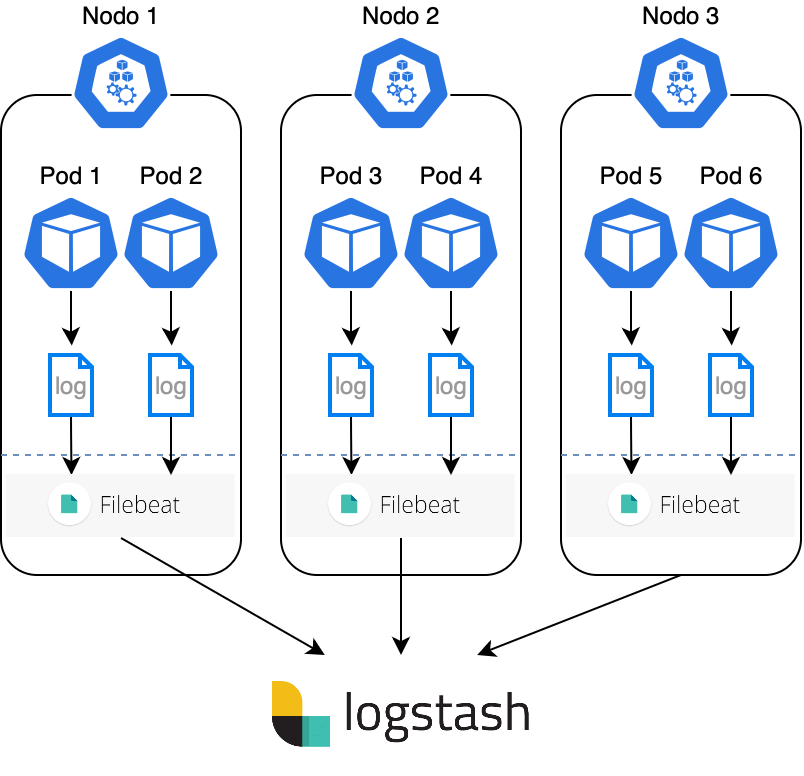
\includegraphics[width=0.75\linewidth]{immagini/capitolo3/filebeat.png}
    \caption{Funzionamento di Filebeat in un cluster multi-nodo.}
    \label{fig:filebeat_multinode}
\end{figure}

\begin{lstlisting}[caption={File di configurazione di Filebeat.},label=lst:filebeat-conf, keywordstyle=\color{black}, commentstyle=\color{black},stringstyle=\color{black},numberstyle=\color{black}]
filebeat.inputs:
- type: container
  paths:
  - /var/log/containers/*.log
processors:
  - add_kubernetes_metadata:
      host: ${NODE_NAME}
      matchers:
      - logs_path:
          logs_path: "/var/log/containers/"
  - drop_event.when.not.or:
    - contains.kubernetes.namespace: "log-enabled"
output.logstash:
  hosts: ['${LOGSTASH_HOSTS}']
\end{lstlisting}

Per gli scopi di questa tesi, Filebeat può essere configurato come mostrato in Codice \ref{lst:filebeat-conf}:
\paragraph{Filebeat.inputs}
La sezione \texttt{filebeat.inputs} specifica gli ingressi per Filebeat. Questi ingressi sono configurati per raccogliere dati dal tipo \myenquote{container}. In particolare, Filebeat è configurato per monitorare tutti i file di log nella directory \texttt{/var/log/containers/} con estensione \texttt{.log}.

\paragraph{Processors}
La sezione \texttt{processors} definisce una serie di processori che vengono applicati agli eventi raccolti da Filebeat. Il primo processore, \texttt{add\_kubernetes\_metadata}, è utilizzato per arricchire gli eventi con metadati di Kubernetes. Utilizza il nome del nodo host, specificato dalla variabile \texttt{\${NODE\_NAME}}, per ottenere questi metadati. Per determinare a quali eventi applicare questi metadati, il processore utilizza un criterio di corrispondenza basato sul percorso dei log, specificando il percorso \texttt{"/var/log/containers/"}.

Il secondo processore, \texttt{drop\_event}, ha la funzione di eliminare certi eventi basati su condizioni specificate. In questo caso, l'evento verrà scartato se non contiene il namespace di Kubernetes \texttt{log-enabled}, ovvero il namespace che conterrà il deployment target da analizzare.

\paragraph{Output.logstash}
La sezione \texttt{output.logstash} stabilisce come gli eventi raccolti da Filebeat devono essere inoltrati. In particolare, gli eventi vengono inviati a Logstash. Gli host di destinazione per Logstash sono specificati dalla variabile \texttt{\${LOGSTASH\_HOSTS}}.

\subsection{Configurazione di Logstash}\label{subsect:Configurazione di Logstash}
Logstash viene usato e configurato per elaborare opportunamente gli access log generati. In particolare, l'utilizzo principale dell'istanza di Logstash aggiunto al deployment di un'applicazione risiede nell'uniformare log che arrivano dalle varie istanze di Filebeat in modo da memorizzarli tutti nello stesso formato JSON.


Nel Codice \ref{lst:logstash-conf}, viene mostrato come configurare un'istanza di Logstash per assolvere agli scopi descritti sopra:
\begin{lstlisting}[caption={File di configurazione di Logstash.},label=lst:logstash-conf, keywordstyle=\color{black}, commentstyle=\color{black},stringstyle=\color{black},numberstyle=\color{black}]
input {
  beats {
    port => 5044
  }
}
filter {
  if [message] =~ /^{.*}$/ {
    json {
      source => "message"
      tag_on_failure => ["_jsonparsefailure"]
    }
  }
}
output {
  ElasticSearch {
    hosts => "${ElasticSearch_HOSTS}"
    index => "logstash-%{+YYYY.MM.dd}"
  }
}
\end{lstlisting}

\paragraph{Input}

Nella sezione di \texttt{input}, l'unica linea presente imposta Logstash per accettare eventi dall'istanza Filebeat sulla porta 5044.

\paragraph{Filter}

La sezione \texttt{filter} viene utilizzata per processare e trasformare gli eventi che attraversano Logstash prima che vengano inviati all'output. In questa configurazione specifica, c'è un filtro condizionale che verifica se il campo \texttt{message} di un evento contiene una stringa JSON (identificata dalla presenza di parentesi graffe all'inizio e alla fine della stringa). Se la condizione viene soddisfatta, il filtro \texttt{json} viene applicato per analizzare il campo \texttt{message} e convertirlo in un oggetto JSON strutturato. Se l'analisi fallisce, viene applicato un tag \texttt{\_jsonparsefailure} all'evento, il che può aiutare nella diagnostica e nel troubleshooting.

\paragraph{Output}

Nella sezione \texttt{output}, gli eventi processati sono inviati all'istanza ElasticSearch. Questa configurazione specifica l'endpoint di ElasticSearch utilizzando la variabile di ambiente \texttt{ElasticSearch\_HOSTS} (definita nel file di deployment di ElasticSearch). Gli eventi sono poi indicizzati in indici con un formato di nome specifico, \texttt{logstash-\%{+YYYY.MM.dd}}, che suddivide gli eventi in base alla data in cui sono stati ricevuti. Questo schema di naming consente di gestire facilmente la rotazione e la conservazione dei dati nel tempo.

\section{Architettura risultante dalla configurazione proposta}

La Figura \ref{fig:full_diagram} fornisce una visuale completa dell'architettura risultante dalla configurazione proposta, per il deployment di due servizi in un cluster Kubernetes. I due servizi sono dispiegati in due container separati, ciascuno eseguito in un pod separato. I pod sono equipaggiati con proxy Envoy, gestiti da Istio e configurati in modo da emettere gli access log come descritto nella Sezione 3.2. I log emessi dal container e dal proxy Envoy in ciascun pod sono prelevati da Filebeat e mandati a Logstash. Quest’ultimo procede alla loro conversione nel formato unificato e li spedisce ad ElasticSearch, il quale li memorizza. L’accesso ai log memorizzati può essere fatto tramite l’interfaccia offerta da Kibana, ma anche scaricando un dump dei log memorizzati direttamente da ElasticSearch.

\begin{figure}[h]
    \centering
    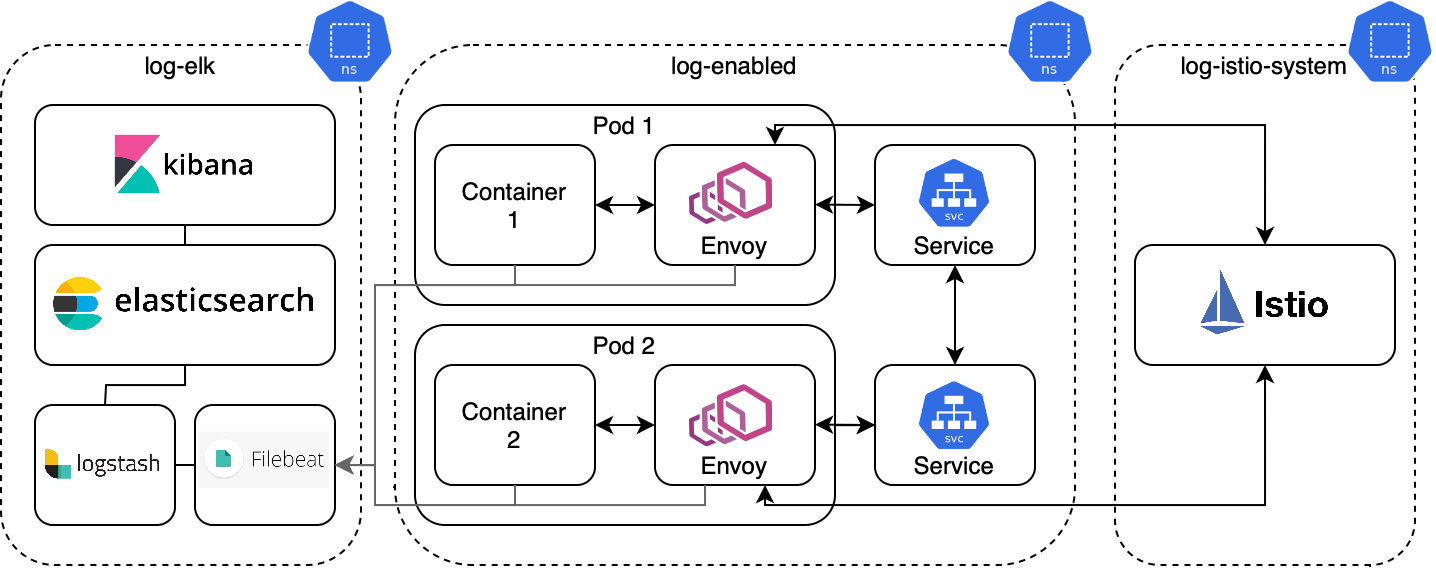
\includegraphics[width=1\linewidth]{immagini/capitolo3/full_diagram.png}
    \caption{Diagramma completo dell'architettura del sistema.}
    \label{fig:full_diagram}
\end{figure}